%%% Research Diary - Entry
\documentclass[11pt,letterpaper]{article}

% Working date: The date this entry is describing. Not necessary the date of last edit.
\newcommand{\workingDate}{\textsc{  2012 $|$ 3 $|$ 12 } }

% Name and institution must preceed call to researchdiary.sty package
\newcommand{\userName}{ BW Keller }
\newcommand{\institution}{ McMaster University }

% The guts and glory
\usepackage{research_diary}
\setcounter{secnumdepth}{-1}

% Begin document
\begin{document}

\section{To Do}
\begin{bullets}
\item[\checkmark] Generate Tipsy files from Oscar's ICs
\item Rewrite Chris' density profile code to generate SPH ICs
\end{bullets}

\textleaf : \textit{In Progress} \qquad \checkmark : \textit{Completed}
\section{Daily Log}

\subsection{Thursday}

Today I finally finished building the tipsy generator that generates ICs
from Oscar's disk tables. The final derivation for the temperature from
the specific internal energy was as follows:
\[T = \frac{2}{3}\frac{u\mu m_H}{k_B}\] The units for the specific
internal energy are simply the squared velocity units: $km^2/s^2$. I
also assumed that the gas had the same mean molecular weight as the sun,
$\mu = 0.6$. This gives me a pretty reasonable looking temperature
profile:

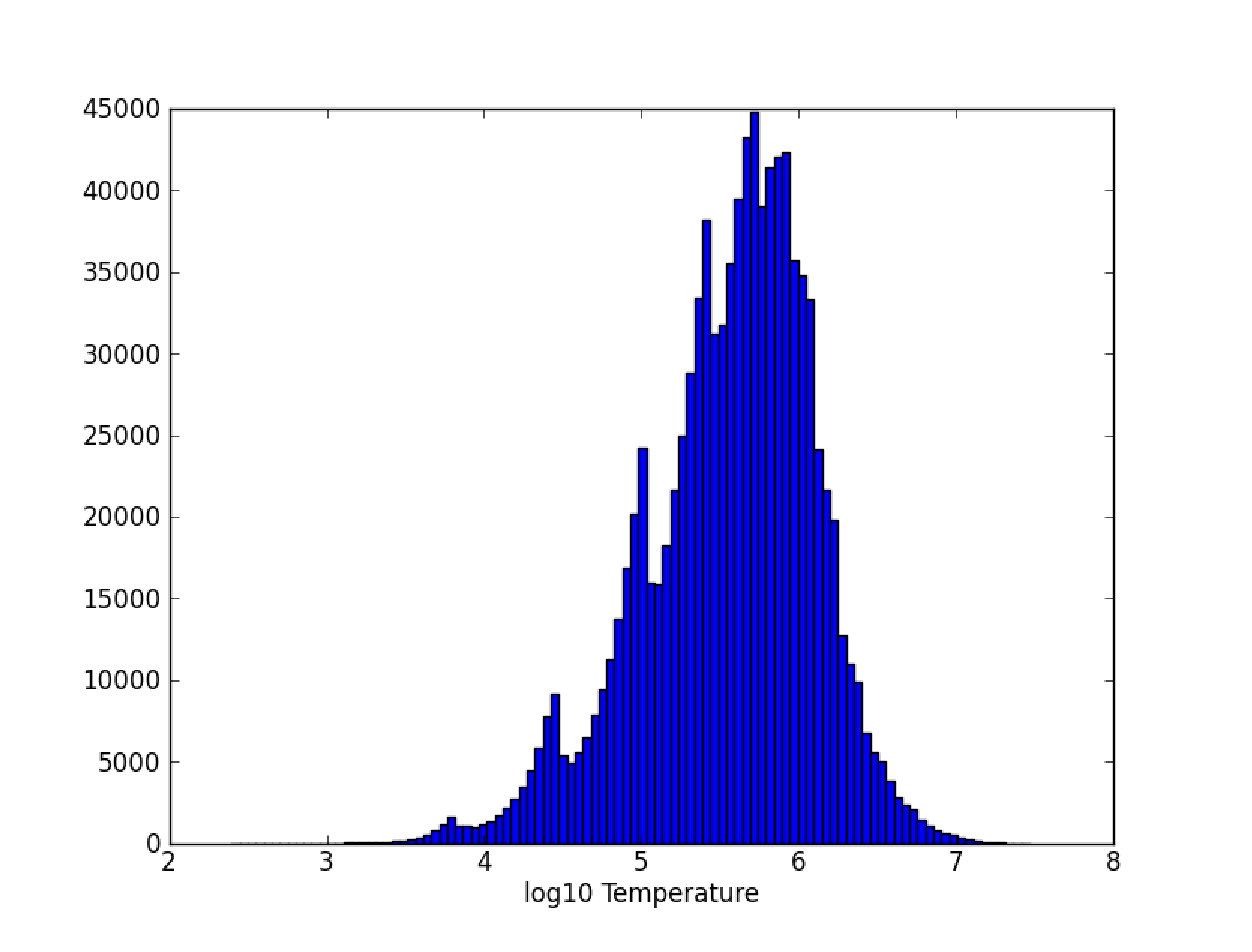
\includegraphics[width=0.9\textwidth]{oscar_disk_temperature_histogram}

The group meeting was also very interesting today. I'm going to work
with Chris to produce a direct comparison of his work using SPH as a way
of checking his work and also testing the new ionization feedback. I
need to take Chris's code for generating the vertical density profile,
and ``stretch'' a glass to fit this density profile. I'll need to talk
to James, Patrick, and Chris about doing this. The final IC product will
have to tile the glass cubes on top of each other, and then do the
stretching. I've found a paper by Dieh et al. \emph{Generating Optimal
Initial Conditions for SPH Simulations} that seems to describe this
process, that I will read today or tomorrow that should illuminate this
process.


\end{document}